\documentclass{article}

% content/resources/templates/preamble.tex
\usepackage[margin=0.6in]{geometry}
\author{Milav Dabgar}
\usepackage{amsmath,amssymb,amsthm}
\usepackage{booktabs}
\usepackage{multirow}
\usepackage{xcolor}
\usepackage{tcolorbox}
\tcbuselibrary{breakable,skins}
\usepackage[colorlinks=true,linkcolor=blue]{hyperref}
\usepackage{titlesec}
\usepackage{enumitem}
\usepackage{tikz}
\usepackage{pgfplots}
\usepackage{circuitikz}
\usepackage[version=4]{mhchem}
\usepackage{longtable}
\usepackage{array}
\usepackage{float}
\usepackage{caption}
\usepackage{listings}

\lstset{
  basicstyle=\small\ttfamily,
  breaklines=true,
  breakatwhitespace=false,
  postbreak=\mbox{\textcolor{red}{$\hookrightarrow$}\space},
  float=false,
  numbers=left,
  numberstyle=\tiny\color{gray},
  numbersep=10pt,
  xleftmargin=2em,
  keywordstyle=\color{blue},
  commentstyle=\color{green!60!black},
  stringstyle=\color{purple},
  backgroundcolor=\color{gray!5},
  showstringspaces=false,
  tabsize=2,
  captionpos=b,
  keepspaces=true,
  columns=flexible
}

\pgfplotsset{compat=1.18}
\usetikzlibrary{shapes,arrows,positioning,calc,patterns,decorations.pathmorphing,decorations.markings,arrows.meta}

% Color scheme
\definecolor{headcolor}{RGB}{0,102,204}
\definecolor{keycolor}{RGB}{220,20,60}
\definecolor{solutioncolor}{RGB}{34,139,34}
\definecolor{mnemoniccolor}{RGB}{148,0,211}
\definecolor{codecolor}{RGB}{0,0,100}

% Spacing
\setlength{\parskip}{3pt}
\setlist[itemize]{nosep}
\setlist[enumerate]{nosep}

% Title formatting
\titleformat{\section}{\Large\bfseries\color{headcolor}}{\thesection}{1em}{}
\titleformat{\subsection}{\large\bfseries\color{headcolor}}{\thesubsection}{1em}{}

% Pandoc tightlist compatibility
\providecommand{\tightlist}{%
  \setlength{\itemsep}{0pt}\setlength{\parskip}{0pt}}

% Pandoc longtable compatibility
\newcounter{none}
\def\thenone{}


% content/resources/templates/english-boxes.tex
% This file is currently empty - it exists to maintain consistency with the import structure.
% Add custom environments here if needed in the future.


% Custom commands for GTU solutions
% This file defines semantic commands for consistent formatting

% Question command with automatic formatting
\newcommand{\question}[2]{%
  \section*{Question #1}%
  \textbf{#2}%
}

% OR question variant
\newcommand{\questionor}[2]{%
  \section*{Question #1 OR}%
  \textbf{#2}%
}

% Proper table environment with caption
\newenvironment{answertable}[1]{%
  \begin{table}[htbp]
  \centering
  \caption{#1}
}{%
  \end{table}
}

% Proper figure environment for diagrams
\newenvironment{answerdiagram}[1]{%
  \begin{figure}[htbp]
  \centering
  \caption{#1}
}{%
  \end{figure}
}

% Semantic markup for key terms
\newcommand{\keyword}[1]{\textbf{#1}}
\newcommand{\code}[1]{\texttt{#1}}
\newcommand{\classname}[1]{\texttt{#1}}
\newcommand{\methodname}[1]{\texttt{#1}}

% Proper quotation marks
\newcommand{\mnemonic}[1]{``#1''}


\title{Fundamentals of Electronics (4311102) - Summer 2024 Solution}
\date{June 21, 2024}


% \usetikzlibrary{circuits.ee.IEC} removed

\newcommand{\mysolutionbox}[3]{%
    \noindent\textbf{#1: #2}%
    \begin{solutionbox}
    #3
    \end{solutionbox}%
    \vspace{0.5em}
}

\begin{document}
\maketitle

\questionmarks{Question 1}{14}{}
\textbf{Answer any seven out of ten.}

\mysolutionbox{Question 1(1)}{Define resistor and give its unit.}{
    A \keyword{resistor} is an electronic component that opposes the flow of electric current. Its unit is \keyword{Ohm} ($\Omega$).

    \captionof{table}{Resistor Properties}
    \begin{tabulary}{\linewidth}{|L|L|}
    \hline
    \textbf{Property} & \textbf{Description} \\
    \hline
    Symbol & {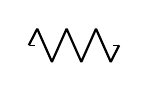
\begin{tikzpicture}[baseline=-0.3em] \draw (0,0) to[R] (1,0); \end{tikzpicture}} \\
    \hline
    Unit & Ohm ($\Omega$) \\
    \hline
    Function & Limits current flow \\
    \hline
    \end{tabulary}

    \begin{mnemonicbox}
    \mnemonic{Resistors Oppose Current (ROC)}
    \end{mnemonicbox}
}

\mysolutionbox{Question 1(2)}{Give two examples of active and passive components each.}{
    \captionof{table}{Electronic Components Classification}
    \begin{tabulary}{\linewidth}{|L|L|}
    \hline
    \textbf{Active Components} & \textbf{Passive Components} \\
    \hline
    1. Transistors & 1. Resistors \\
    2. Diodes & 2. Capacitors \\
    \hline
    \end{tabulary}

    \begin{mnemonicbox}
    \mnemonic{TARD - Transistors And Resistors Differ}
    \end{mnemonicbox}
}

\mysolutionbox{Question 1(3)}{Draw symbols of any two semiconductor devices.}{
    \begin{answerdiagram}{Semiconductor Device Symbols}
    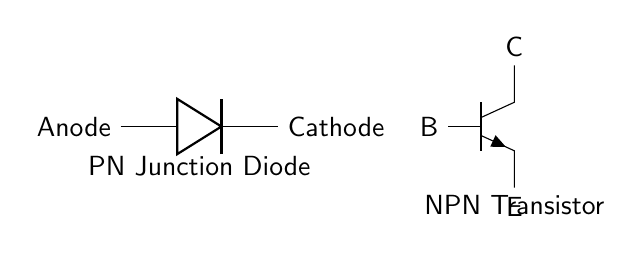
\begin{tikzpicture}[, font=\sffamily]
        % Diode
        \draw (0,0) node[anchor=east] {Anode} to[diode] (2,0) node[anchor=west] {Cathode};
        \node at (1, -0.5) {PN Junction Diode};

        % NPN Transistor
        \begin{scope}[xshift=5cm, yshift=0cm]
            \draw (0,0) node[npn] (t1) {};
            \node[left] at (t1.B) {B};
            \node[above] at (t1.C) {C};
            \node[below] at (t1.E) {E};
            \node at (0, -1) {NPN Transistor};
        \end{scope}
    \end{tikzpicture}
    \end{answerdiagram}

    \begin{mnemonicbox}
    \mnemonic{Diodes Direct, Transistors Transfer}
    \end{mnemonicbox}
}

\mysolutionbox{Question 1(4)}{Differentiate between intrinsic and extrinsic semiconductor.}{
    \captionof{table}{Intrinsic vs Extrinsic Semiconductors}
    \begin{tabulary}{\linewidth}{|L|L|}
    \hline
    \textbf{Intrinsic} & \textbf{Extrinsic} \\
    \hline
    Pure semiconductor without impurities & Semiconductor with added impurities \\
    \hline
    Equal number of holes and electrons & Unequal holes and electrons \\
    \hline
    Examples: Pure Silicon, Germanium & Examples: Silicon doped with Phosphorus \\
    \hline
    \end{tabulary}

    \begin{mnemonicbox}
    \mnemonic{Pure In, Doped Ex}
    \end{mnemonicbox}
}

\mysolutionbox{Question 1(5)}{LED stands for \_\_\_\_\_\_\_\_\_\_\_\_\_\_\_\_\_.}{
    LED stands for \textbf{Light Emitting Diode}.

    \begin{answerdiagram}{LED Symbol}
    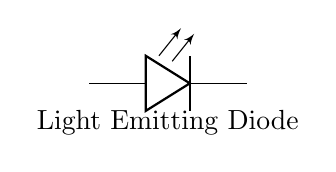
\begin{tikzpicture}[]
        \draw (0,0) to[leDo] (2,0);
        \node at (1, -0.5) {Light Emitting Diode};
    \end{tikzpicture}
    \end{answerdiagram}

    \begin{mnemonicbox}
    \mnemonic{Light Emitters Dazzle}
    \end{mnemonicbox}
}

\mysolutionbox{Question 1(6)}{State any two applications of Photo-diode.}{
    \captionof{table}{Photo-diode Applications}
    \begin{tabulary}{\linewidth}{|L|L|}
    \hline
    \textbf{Application} & \textbf{How it works} \\
    \hline
    Light sensors & Converts light to electrical current \\
    \hline
    Optical communication & Detects optical signals in fiber optics \\
    \hline
    \end{tabulary}

    \begin{mnemonicbox}
    \mnemonic{Light Sensing Communication (LSC)}
    \end{mnemonicbox}
}

\mysolutionbox{Question 1(7)}{List the types of transistor and draw their symbols.}{
    \textbf{Types of Transistors:}
    \begin{enumerate}
        \item NPN Transistor
        \item PNP Transistor
    \end{enumerate}

    \begin{answerdiagram}{Transistor Symbols}
    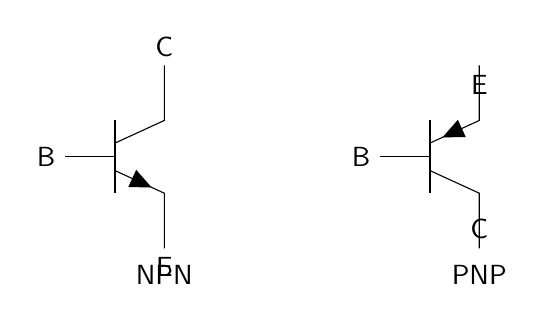
\begin{tikzpicture}[, font=\sffamily]
        % NPN
        \begin{scope}[xshift=0cm]
            \draw (0,0) node[npn, xscale=1.5, yscale=1.5] (npn) {};
            \node[left] at (npn.B) {B};
            \node[above] at (npn.C) {C};
            \node[below] at (npn.E) {E};
            \node at (0, -1.5) {NPN};
        \end{scope}

        % PNP
        \begin{scope}[xshift=4cm]
            \draw (0,0) node[pnp, xscale=1.5, yscale=1.5] (pnp) {};
            \node[left] at (pnp.B) {B};
            \node[above] at (pnp.C) {C};
            \node[below] at (pnp.E) {E};
            \node at (0, -1.5) {PNP};
        \end{scope}
    \end{tikzpicture}
    \end{answerdiagram}

    \begin{mnemonicbox}
    \mnemonic{Not Pointing iN, Pointing outP}
    \end{mnemonicbox}
}

\mysolutionbox{Question 1(8)}{Give the value of forward voltage drop of Germanium and Silicon diode.}{
    \captionof{table}{Forward Voltage Drop Values}
    \begin{tabulary}{\linewidth}{|L|L|}
    \hline
    \textbf{Diode Type} & \textbf{Forward Voltage Drop} \\
    \hline
    Germanium & 0.3V \\
    \hline
    Silicon & 0.7V \\
    \hline
    \end{tabulary}

    \begin{mnemonicbox}
    \mnemonic{Germanium's Three, Silicon's Seven (0.3V, 0.7V)}
    \end{mnemonicbox}
}

\mysolutionbox{Question 1(9)}{The \_\_\_\_\_\_\_\_\_\_\_\_\_\_\_\_\_ diode can be used as a light detector.}{
    The \textbf{Photodiode} can be used as a light detector.

    \begin{answerdiagram}{Photodiode Symbol}
    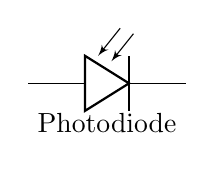
\begin{tikzpicture}[]
        \draw (0,0) to[photodiode] (2,0);
        \node at (1, -0.5) {Photodiode};
    \end{tikzpicture}
    \end{answerdiagram}

    \begin{mnemonicbox}
    \mnemonic{Photo Detects Light (PDL)}
    \end{mnemonicbox}
}

\mysolutionbox{Question 1(10)}{Define Q-factor of a coil.}{
    \keyword{Q-factor} (Quality factor) of a coil is the ratio of its inductive reactance to its resistance, indicating how efficiently it stores energy.

    \captionof{table}{Q-Factor}
    \begin{tabulary}{\linewidth}{|L|L|}
    \hline
    \textbf{Parameter} & \textbf{Description} \\
    \hline
    Formula & $Q = \frac{X_L}{R}$ \\
    \hline
    Higher Q & Better quality, less energy loss \\
    \hline
    Lower Q & Poor quality, more energy loss \\
    \hline
    \end{tabulary}

    \begin{mnemonicbox}
    \mnemonic{Quality equals Reactance over Resistance (QRR)}
    \end{mnemonicbox}
}

\questionmarks{Question 2(a)}{3}{}
\mysolutionbox{Question 2(a)}{Explain colour coding method of resistor.}{
    Resistor color coding uses colored bands to indicate resistance value and tolerance.

    \captionof{table}{Resistor Color Code}
    \begin{tabulary}{\linewidth}{|L|L|L|}
    \hline
    \textbf{Color} & \textbf{Digit} & \textbf{Multiplier} \\
    \hline
    Black & 0 & $10^0$ \\
    \hline
    Brown & 1 & $10^1$ \\
    \hline
    Red & 2 & $10^2$ \\
    \hline
    Orange & 3 & $10^3$ \\
    \hline
    Yellow & 4 & $10^4$ \\
    \hline
    Green & 5 & $10^5$ \\
    \hline
    Blue & 6 & $10^6$ \\
    \hline
    Violet & 7 & $10^7$ \\
    \hline
    Grey & 8 & $10^8$ \\
    \hline
    White & 9 & $10^9$ \\
    \hline
    \end{tabulary}

    \vspace{1em}
    \textbf{For a 4-band resistor:}
    \begin{itemize}
        \item First band: First digit
        \item Second band: Second digit
        \item Third band: Multiplier
        \item Fourth band: Tolerance
    \end{itemize}

    \begin{mnemonicbox}
    \mnemonic{Bad Boys Race Our Young Girls But Violet Generally Wins (Black, Brown, Red, Orange, Yellow, Green, Blue, Violet, Grey, White)}
    \end{mnemonicbox}
}

\mysolutionbox{Question 2(a) OR}{Explain Light Dependent Resistor with its characteristics.}{
    \keyword{LDR} is a resistor whose resistance decreases when light intensity increases.

    \textbf{Characteristics:}
    \captionof{table}{LDR Properties}
    \begin{tabulary}{\linewidth}{|L|L|}
    \hline
    \textbf{Parameter} & \textbf{Behavior} \\
    \hline
    Dark condition & High resistance ($M\Omega$) \\
    \hline
    Bright condition & Low resistance ($k\Omega$) \\
    \hline
    Response time & Few milliseconds \\
    \hline
    \end{tabulary}

    \begin{answerdiagram}{LDR Characteristics}
    \begin{tikzpicture}
        \begin{axis}[
            gtu plot,
            xlabel={Light Intensity (Lux)},
            ylabel={Resistance ($\Omega$)},
            domain=0:100,
            xmin=0, xmax=100,
            ymin=0, ymax=100,
            xtick={0,50,100},
            ytick={0,50,100},
            axis lines=left,
        ]
        \addplot[thick, blue, smooth] coordinates {(5, 90) (20, 40) (50, 20) (90, 10)};
        \end{axis}
    \end{tikzpicture}
    \end{answerdiagram}

    \begin{mnemonicbox}
    \mnemonic{Light Up, Resistance Down (LURD)}
    \end{mnemonicbox}
}

\questionmarks{Question 2(b)}{3}{}
\mysolutionbox{Question 2(b)}{Explain classification of capacitors in detail.}{
    Capacitors are classified based on dielectric material and construction.

    \begin{answerdiagram}{Classification of Capacitors}
    \begin{tikzpicture}[edge from parent/.style={draw, -latex}, level distance=1.5cm, sibling distance=2.5cm]
        \node[gtu block] {Capacitors}
            child {node[gtu block, align=center] {Fixed\\Capacitors}
                child {node[gtu block] {Ceramic}}
                child {node[gtu block] {Electrolytic}}
                child {node[gtu block] {Polyester}}
            }
            child {node[gtu block, align=center] {Variable\\Capacitors}
                child {node[gtu block] {Air Gang}}
                child {node[gtu block] {Trimmer}}
            };
    \end{tikzpicture}
    \end{answerdiagram}

    \captionof{table}{Capacitor Classifications}
    \begin{tabulary}{\linewidth}{|L|L|L|}
    \hline
    \textbf{Type} & \textbf{Dielectric} & \textbf{Applications} \\
    \hline
    Ceramic & Ceramic & High frequency \\
    \hline
    Electrolytic & Aluminum oxide & Power supplies \\
    \hline
    Polyester & Plastic film & General purpose \\
    \hline
    Tantalum & Tantalum oxide & Small, high capacity \\
    \hline
    \end{tabulary}

    \begin{mnemonicbox}
    \mnemonic{CEPT (Ceramic, Electrolytic, Polyester, Tantalum)}
    \end{mnemonicbox}
}

\mysolutionbox{Question 2(b) OR}{Explain classification of inductor in detail.}{
    Inductors are classified based on core material and construction.

    \begin{answerdiagram}{Classification of Inductors}
    \begin{tikzpicture}[edge from parent/.style={draw, -latex}, level distance=1.5cm, sibling distance=2.5cm]
        \node[gtu block] {Inductors}
            child {node[gtu block] {Air Core}}
            child {node[gtu block] {Iron Core}}
            child {node[gtu block] {Ferrite Core}}
            child {node[gtu block] {Toroidal}};
    \end{tikzpicture}
    \end{answerdiagram}

    \captionof{table}{Inductor Classifications}
    \begin{tabulary}{\linewidth}{|L|L|L|}
    \hline
    \textbf{Type} & \textbf{Core} & \textbf{Characteristics} \\
    \hline
    Air core & Air & Low inductance, low losses \\
    \hline
    Iron core & Iron & High inductance, high losses \\
    \hline
    Ferrite core & Ferrite & Medium inductance, low losses \\
    \hline
    Toroidal & Ring shaped & High efficiency, low EMI \\
    \hline
    \end{tabulary}

    \begin{mnemonicbox}
    \mnemonic{Air Iron Ferrite Toroid (AIFT)}
    \end{mnemonicbox}
}

\questionmarks{Question 2(c)}{4}{}
\mysolutionbox{Question 2(c)}{State and explain Faraday's laws of Electromagnetic Induction.}{
    Faraday's laws explain how electromagnetic induction works.

    \textbf{Faraday's First Law:}
    When a magnetic field linked with a conductor changes, an EMF is induced in the conductor.

    \textbf{Faraday's Second Law:}
    The magnitude of induced EMF is proportional to the rate of change of magnetic flux.

    \captionof{table}{Faraday's Laws Summary}
    \begin{tabulary}{\linewidth}{|L|L|L|}
    \hline
    \textbf{Law} & \textbf{Statement} & \textbf{Formula} \\
    \hline
    First Law & Change in magnetic field induces EMF & - \\
    \hline
    Second Law & EMF $\propto$ rate of change of flux & $E = -N \frac{d\Phi}{dt}$ \\
    \hline
    \end{tabulary}

    \begin{answerdiagram}{Faraday's Law}
    \begin{tikzpicture}
        % Coil
        \draw[decorate, decoration={coil, amplitude=4mm, segment length=3mm, post length=3mm}] (0,0) -- (4,0);
        \draw (4,0) to[galvanometer] (4,-2) -- (0,-2) -- (0,0);
        
        % Magnet
        \draw[fill=red!60] (-3,0.5) rectangle (-1.5, -0.5);
        \node at (-2.6, 0) {N};
        \draw[fill=blue!60] (-1.5,0.5) rectangle (0, -0.5);
        \node at (-0.4, 0) {S};
        
        % Movement arrow
        \draw[->, ultra thick] (-1, 0.8) -- (1, 0.8) node[midway, above] {Motion};
    \end{tikzpicture}
    \end{answerdiagram}

    \begin{mnemonicbox}
    \mnemonic{Change Magnetic Field, Create Electric Current (CMFCEC)}
    \end{mnemonicbox}
}

\mysolutionbox{Question 2(c) OR}{Enlist specifications of capacitors and explain two in detail.}{
    \textbf{Specifications of Capacitors:}
    \begin{enumerate}
        \item Capacitance value
        \item Voltage rating
        \item Tolerance
        \item Leakage current
        \item Temperature coefficient
    \end{enumerate}

    \textbf{Detailed Explanation:}
    
    \textbf{1. Capacitance Value:}
    The amount of charge a capacitor can store per volt, measured in Farads (F).

    \textbf{2. Voltage Rating:}
    The maximum voltage that can be applied without damaging the capacitor.

    \captionof{table}{Capacitor Specifications}
    \begin{tabulary}{\linewidth}{|L|L|L|}
    \hline
    \textbf{Specification} & \textbf{Description} & \textbf{Typical Values} \\
    \hline
    Capacitance & Charge storage capacity & pF to mF \\
    \hline
    Voltage Rating & Maximum safe voltage & 16V, 25V, 50V \\
    \hline
    \end{tabulary}

    \begin{mnemonicbox}
    \mnemonic{Capacitors Very Tolerant of Low Temperatures (CVTLT)}
    \end{mnemonicbox}
}

\questionmarks{Question 2(d)}{4}{}
\mysolutionbox{Question 2(d)}{Write colour band of 47$\Omega\pm$5\% resistance.}{
    For $47\Omega \pm 5\%$ resistor, the color bands are:

    \captionof{table}{Color Bands for 47$\Omega\pm$5\%}
    \begin{tabulary}{\linewidth}{|L|L|L|}
    \hline
    \textbf{Band} & \textbf{Color} & \textbf{Represents} \\
    \hline
    1st band & Yellow & 4 \\
    \hline
    2nd band & Violet & 7 \\
    \hline
    3rd band & Black & $\times 10^0$ \\
    \hline
    4th band & Gold & $\pm 5\%$ \\
    \hline
    \end{tabulary}

    \begin{answerdiagram}{Resistor Color Code: 47 $\pm$ 5\%}
    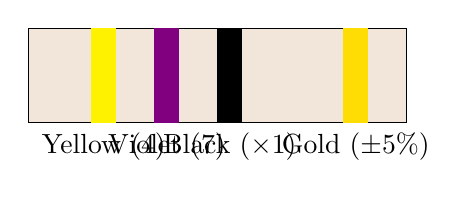
\begin{tikzpicture}[scale=0.8]
        \draw[fill=brown!20] (0,0) rectangle (6,1.5);
        \fill[yellow] (1,0) rectangle (1.4,1.5); % Yellow
        \fill[violet] (2,0) rectangle (2.4,1.5); % Violet
        \fill[black] (3,0) rectangle (3.4,1.5); % Black
        \fill[yellow!80!orange] (5,0) rectangle (5.4,1.5); % Gold
        
        \node[below] at (1.2,0) {Yellow (4)};
        \node[below] at (2.2,0) {Violet (7)};
        \node[below] at (3.2,0) {Black ($\times 1$)};
        \node[below] at (5.2,0) {Gold ($\pm 5\%$)};
    \end{tikzpicture}
    \end{answerdiagram}

    \begin{mnemonicbox}
    \mnemonic{Yellow Violets Bring Gold}
    \end{mnemonicbox}
}

\mysolutionbox{Question 2(d) OR}{Calculate value of resistor and tolerance for a given colour code: Brown, Black, yellow.}{
    \captionof{table}{Interpretation of Brown, Black, Yellow}
    \begin{tabulary}{\linewidth}{|L|L|L|L|}
    \hline
    \textbf{Band} & \textbf{Color} & \textbf{Value} & \textbf{Meaning} \\
    \hline
    1st & Brown & 1 & First digit \\
    \hline
    2nd & Black & 0 & Second digit \\
    \hline
    3rd & Yellow & $10^4$ & Multiplier \\
    \hline
    \end{tabulary}

    \vspace{1em}
    \textbf{Calculation:}
    \begin{itemize}
        \item 1st digit: 1
        \item 2nd digit: 0
        \item Multiplier: $10^4$
    \end{itemize}
    
    Value = $10 \times 10^4 = 100,000\Omega = 100 k\Omega$

    No 4th band means $\pm 20\%$ tolerance.

    \begin{answerdiagram}{Resistor: 100k$\Omega$}
    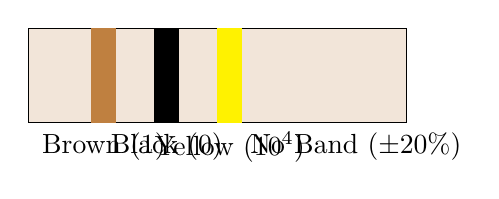
\begin{tikzpicture}[scale=0.8]
        \draw[fill=brown!20] (0,0) rectangle (6,1.5);
        \fill[brown] (1,0) rectangle (1.4,1.5); % Brown
        \fill[black] (2,0) rectangle (2.4,1.5); % Black
        \fill[yellow] (3,0) rectangle (3.4,1.5); % Yellow
        
        \node[below] at (1.2,0) {Brown (1)};
        \node[below] at (2.2,0) {Black (0)};
        \node[below] at (3.2,0) {Yellow ($10^4$)};
        \node[below] at (5.2,0) {No Band ($\pm 20\%$)};
    \end{tikzpicture}
    \end{answerdiagram}

    \begin{mnemonicbox}
    \mnemonic{Big Black Yield (Brown-Black-Yellow)}
    \end{mnemonicbox}
}

\questionmarks{Question 3(a)}{3}{}
\mysolutionbox{Question 3(a)}{Define doping. Give the name of semiconductor materials fabricated by doping with an example of each.}{
    \keyword{Doping} is the process of adding impurities to a pure semiconductor to modify its electrical properties.

    \captionof{table}{Doped Semiconductors}
    \begin{tabulary}{\linewidth}{|L|L|L|L|}
    \hline
    \textbf{Type} & \textbf{Dopant Added} & \textbf{Example} & \textbf{Majority Carriers} \\
    \hline
    P-type & Trivalent (Boron, Gallium) & Silicon + Boron & Holes \\
    \hline
    N-type & Pentavalent (Phosphorus, Arsenic) & Silicon + Phosphorus & Electrons \\
    \hline
    \end{tabulary}

    \begin{answerdiagram}{Doping Process}
    \begin{tikzpicture}[node distance=2.5cm, auto, >=latex]
        \node [gtu block] (pure) {Pure Semiconductor};
        \node [gtu block, below of=pure, xshift=-2.5cm] (ptype) {P-type};
        \node [gtu block, below of=pure, xshift=2.5cm] (ntype) {N-type};
        
        \path [gtu arrow] (pure) -- node [left, align=center] {Add Trivalent\\Impurity} (ptype);
        \path [gtu arrow] (pure) -- node [right, align=center] {Add Pentavalent\\Impurity} (ntype);
    \end{tikzpicture}
    \end{answerdiagram}

    \begin{mnemonicbox}
    \mnemonic{Positive has Plus Holes, Negative has Numerous Electrons (PHNE)}
    \end{mnemonicbox}
}

\mysolutionbox{Question 3(a) OR}{Define Ripple factor, Peak Inverse Voltage (PIV), Rectification efficiency.}{
    \captionof{table}{Rectifier Terms}
    \begin{tabulary}{\linewidth}{|L|L|L|}
    \hline
    \textbf{Term} & \textbf{Definition} & \textbf{Formula} \\
    \hline
    Ripple Factor & Measure of AC component in DC output & $r = \frac{V_{rms(AC)}}{V_{dc}}$ \\
    \hline
    Peak Inverse Voltage & Max reverse voltage diode can withstand & - \\
    \hline
    Rectification Efficiency & Ratio of DC output to AC input power & $\eta = \frac{P_{dc}}{P_{ac}} \times 100\%$ \\
    \hline
    \end{tabulary}

    \begin{mnemonicbox}
    \mnemonic{Ripples Peak Efficiently (RPE)}
    \end{mnemonicbox}
}

\questionmarks{Question 3(b)}{3}{}
\mysolutionbox{Question 3(b)}{Explain working of Crystal diode.}{
    A \keyword{Crystal Diode} is a point-contact diode used for detecting RF signals.

    \textbf{Construction}: It consists of a semiconductor crystal (Germanium/Silicon) and a thin tungsten wire (cat's whisker) pressing against it.
    
    \textbf{Function}: It rectifies high-frequency radio signals (demodulation).

    \begin{answerdiagram}{Crystal Diode Construction}
    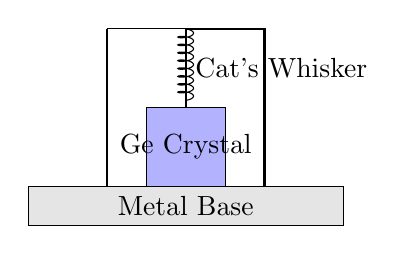
\begin{tikzpicture}
        \draw[fill=gray!20] (0,0) rectangle (4,0.5); % Base
        \node at (2,0.25) {Metal Base};
        \draw[fill=blue!30] (1.5,0.5) rectangle (2.5,1.5); % Crystal
        \node at (2,1) {Ge Crystal};
        \draw[thick] (2,1.5) -- (2,2.5) -- (3,2.5) -- (3,0.5); % Whisker visualization (schematic)
        \draw[decorate, decoration={coil, aspect=0.3, segment length=1mm, amplitude=1mm}] (2,2.5) -- (2,1.5);
        \node[right] at (2,2) {Cat's Whisker};
        \draw (1,0.5) -- (1,2.5); % Case enclosure schematic
        \draw (3,0.5) -- (3,2.5);
        \draw (1,2.5) -- (3,2.5);
    \end{tikzpicture}
    \end{answerdiagram}

    \begin{mnemonicbox}
    \mnemonic{Crystal Detects Radio Frequencies (CDRF)}
    \end{mnemonicbox}
}

\mysolutionbox{Question 3(b) OR}{Explain working of photodiode.}{
    \keyword{Photodiode} converts light energy into electrical current when operated in reverse bias.

    \textbf{Working:}
    \begin{enumerate}
        \item Light strikes the PN junction.
        \item Photons generate electron-hole pairs.
        \item Reverse bias field sweeps carriers across junction, creating a current.
    \end{enumerate}

    \begin{answerdiagram}{Photodiode Operation}
    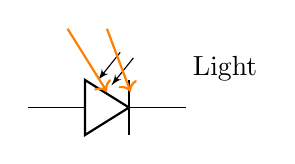
\begin{tikzpicture}[]
        \draw (0,0) to[photodiode] (2,0);
        \draw[->, thick, orange] (0.5, 1) -- (1, 0.2);
        \draw[->, thick, orange] (1.0, 1) -- (1.3, 0.2);
        \node at (2.5, 0.5) {Light};
    \end{tikzpicture}
    \end{answerdiagram}

    \begin{mnemonicbox}
    \mnemonic{Light In, Current Out (LICO)}
    \end{mnemonicbox}
}

\questionmarks{Question 3(c)}{4}{}
\mysolutionbox{Question 3(c)}{Explain half-wave rectifier with circuit diagram and waveforms.}{
    \keyword{Half-wave rectifier} converts AC to pulsating DC by conducting only during positive half cycles.

    \begin{answerdiagram}{Half-Wave Rectifier Circuit}
    \begin{tikzpicture}[]
        \draw (0,2) to[AC source, l={AC Input}] (0,0);
        \draw (0,2) to[diode] (3,2) to[resistor, l={Load}] (3,0) -- (0,0);
    \end{tikzpicture}
    \end{answerdiagram}

    \begin{answerdiagram}{Half-Wave Waveforms}
    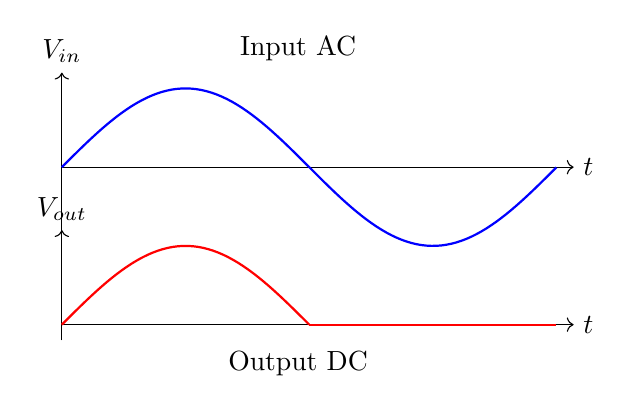
\begin{tikzpicture}
        \begin{scope}[yshift=2cm]
            \draw[->] (0,0) -- (6.5,0) node[right] {$t$};
            \draw[->] (0,-1.2) -- (0,1.2) node[above] {$V_{in}$};
            \draw[thick, blue] plot[domain=0:6.28, samples=100] (\x, {sin(\x r)});
            \node at (3,1.5) {Input AC};
        \end{scope}
        
        \begin{scope}[yshift=0cm]
            \draw[->] (0,0) -- (6.5,0) node[right] {$t$};
            \draw[->] (0,-0.2) -- (0,1.2) node[above] {$V_{out}$};
            \draw[thick, red] plot[domain=0:3.14, samples=50] (\x, {sin(\x r)});
            \draw[thick, red] (3.14,0) -- (6.28,0);
            \node at (3,-0.5) {Output DC};
        \end{scope}
    \end{tikzpicture}
    \end{answerdiagram}

    \begin{mnemonicbox}
    \mnemonic{Half Wave Passes Half (HWPH)}
    \end{mnemonicbox}
}

\mysolutionbox{Question 3(c) OR}{Explain full-wave rectifier with circuit diagram and waveforms.}{
    \keyword{Full-wave rectifier} (Bridge Type) converts both halves of AC input to DC.

    \begin{answerdiagram}{Bridge Rectifier Circuit}
    \begin{tikzpicture}[]
        \draw (0,0) to[AC source, l={Input}] (0,3);
        \draw (2,1.5) to[diode] (3.5,3) to[diode] (5,1.5) to[diode] (3.5,0) to[diode] (2,1.5);
        \draw (0,3) -- (3.5,3);
        \draw (0,0) -- (3.5,0);
        \draw (2,1.5) -- (2,1.5) to[resistor, l={$R_L$}] (5,1.5); 
        % Simplified bridge drawing for clarity
    \end{tikzpicture}
    \end{answerdiagram}
    
    \begin{answerdiagram}{Full-Wave Waveforms}
    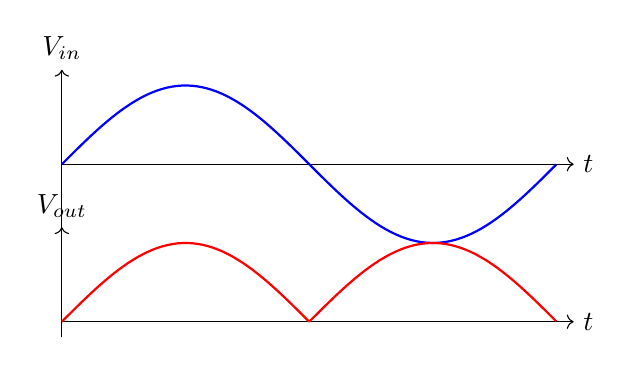
\begin{tikzpicture}
        \begin{scope}[yshift=2cm]
            \draw[->] (0,0) -- (6.5,0) node[right] {$t$};
            \draw[->] (0,-1.2) -- (0,1.2) node[above] {$V_{in}$};
            \draw[thick, blue] plot[domain=0:6.28, samples=100] (\x, {sin(\x r)});
        \end{scope}
        
        \begin{scope}[yshift=0cm]
            \draw[->] (0,0) -- (6.5,0) node[right] {$t$};
            \draw[->] (0,-0.2) -- (0,1.2) node[above] {$V_{out}$};
            \draw[thick, red] plot[domain=0:3.14, samples=50] (\x, {sin(\x r)});
            \draw[thick, red] plot[domain=3.14:6.28, samples=50] (\x, {-sin(\x r)});
        \end{scope}
    \end{tikzpicture}
    \end{answerdiagram}

    \begin{mnemonicbox}
    \mnemonic{Full Wave Makes Full Use (FWMFU)}
    \end{mnemonicbox}
}

\questionmarks{Question 3(d)}{4}{}
\mysolutionbox{Question 3(d)}{Draw and explain VI characteristics of PN junction diode.}{
    \begin{answerdiagram}{VI Characteristics of PN Diode}
    \begin{tikzpicture}
        \begin{axis}[
            gtu plot,
            width=8cm, height=6cm,
            xmin=-10, xmax=1.5,
            ymin=-2, ymax=10,
            axis lines=middle,
            xlabel={$V$ (Volts)},
            ylabel={$I$ (mA)},
            xtick={-10, -5, 0, 0.7},
            xticklabels={-10, -5, 0, 0.7V},
            ytick={0},
        ]
        % Forward
        \addplot[thick, blue, samples=100, domain=0:1] {exp(4*(x-0.7))};
        \node at (axis cs:0.8, 5) {Forward Bias};

        % Reverse
        \addplot[thick, red, samples=100, domain=-9:0] {-0.2};
        \addplot[thick, red] coordinates {(-9, -0.2) (-9, -2)};
        \node at (axis cs:-5, -1) {Reverse Leakage};
        \node at (axis cs:-9.5, -1) {Breakdown};
        \end{axis}
    \end{tikzpicture}
    \end{answerdiagram}

    \textbf{Table: Characteristics}
    \begin{tabulary}{\linewidth}{|L|L|}
    \hline
    \textbf{Region} & \textbf{Behavior} \\
    \hline
    Forward Bias & Current rises exponentially after 0.7V ($V_k$) \\
    \hline
    Reverse Bias & Negligible leakage current \\
    \hline
    Breakdown & Sharp current increase at high reverse voltage \\
    \hline
    \end{tabulary}

    \begin{mnemonicbox}
    \mnemonic{Forward Flows, Reverse Restricts}
    \end{mnemonicbox}
}

\mysolutionbox{Question 3(d) OR}{Write difference between P-type and N-type semiconductor.}{
    \captionof{table}{P-type vs N-type}
    \begin{tabulary}{\linewidth}{|L|L|L|}
    \hline
    \textbf{Property} & \textbf{P-type} & \textbf{N-type} \\
    \hline
    Dopant & Trivalent (Boron) & Pentavalent (Phosphorus) \\
    \hline
    Majority Carriers & Holes & Electrons \\
    \hline
    Minority Carriers & Electrons & Holes \\
    \hline
    \end{tabulary}

    \begin{mnemonicbox}
    \mnemonic{Positive has Plus Holes, Negative has Numerous Electrons}
    \end{mnemonicbox}
}

\questionmarks{Question 4(a)}{3}{}
\mysolutionbox{Question 4(a)}{Explain the principle of operation of LED.}{
    \keyword{LED} works on the principle of \textbf{Electroluminescence}.

    \textbf{Operation:} When forward biased, electrons from N-region recombine with holes in P-region at the junction. This recombination releases energy in the form of photons (light).

    \begin{answerdiagram}{LED Operation}
    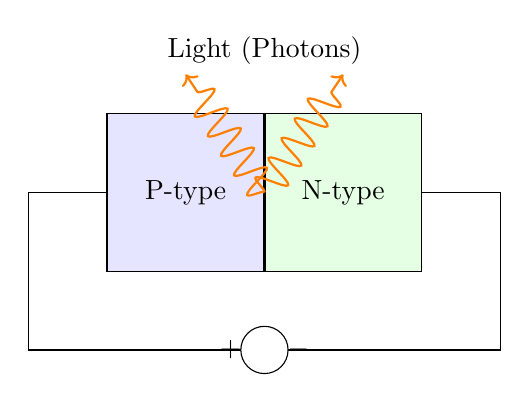
\begin{tikzpicture}
        % PN Block
        \draw[fill=blue!10] (0,0) rectangle (2,2);
        \node at (1,1) {P-type};
        \draw[fill=green!10] (2,0) rectangle (4,2);
        \node at (3,1) {N-type};
        \draw[thick] (2,0) -- (2,2); % Junction

        % Recombination
        \draw[->, decorate, decoration={snake, amplitude=2mm, segment length=3mm, post length=2mm}, orange, thick] (2,1) -- (1,2.5);
        \draw[->, decorate, decoration={snake, amplitude=2mm, segment length=3mm, post length=2mm}, orange, thick] (2,1) -- (3,2.5);
        \node at (2, 2.8) {Light (Photons)};

        % Circuit
        \draw (0,1) -- (-1,1) -- (-1,-1) -- (5,-1) -- (5,1) -- (4,1);
        \draw[fill=white] (2,-1) circle (0.3);
        \node at (2,-1) {$+$ \hspace{1em} $-$};
    \end{tikzpicture}
    \end{answerdiagram}

    \begin{mnemonicbox}
    \mnemonic{Forward Current Emits Light (FCEL)}
    \end{mnemonicbox}
}

\mysolutionbox{Question 4(a) OR}{State applications of LED.}{
    \captionof{table}{LED Applications}
    \begin{tabulary}{\linewidth}{|L|L|}
    \hline
    \textbf{Application} & \textbf{Advantage} \\
    \hline
    Display indicators & Low power \\
    \hline
    Digital displays (7-segment) & Varied colors \\
    \hline
    Lighting (Bulbs) & Energy efficient \\
    \hline
    Remote controls & Infrared communication \\
    \hline
    Traffic signals & High visibility \\
    \hline
    \end{tabulary}
}

\questionmarks{Question 4(b)}{4}{}
\mysolutionbox{Question 4(b)}{Explain Zener diode as voltage regulator.}{
    A \keyword{Zener Diode} maintains a constant output voltage across the load when operated in the reverse breakdown region.

    \begin{answerdiagram}{Zener Voltage Regulator}
    \begin{tikzpicture}[]
        \draw (0,2) node[left] {$V_{in}$} to[resistor, l=$R_S$] (2,2) -- (4,2) -- (4,0) -- (0,0);
        \draw (2,2) to[zener diode, l=$V_Z$] (2,0);
        \draw (4,2) to[resistor, l=$R_L$] (4,0);
        \node[right] at (4,1) {$V_{out} = V_Z$};
    \end{tikzpicture}
    \end{answerdiagram}

    \textbf{Working:}
    \begin{itemize}
        \item The series resistor $R_S$ absorbs voltage fluctuations.
        \item The Zener diode conducts variable current to keep voltage across it constant ($V_Z$).
    \end{itemize}

    \begin{mnemonicbox}
    \mnemonic{Zeners Break to Regulate}
    \end{mnemonicbox}
}

\mysolutionbox{Question 4(b) OR}{Give limitations of zener voltage regulator.}{
    \captionof{table}{Limitations}
    \begin{tabulary}{\linewidth}{|L|L|}
    \hline
    \textbf{Limitation} & \textbf{Effect} \\
    \hline
    Power Dissipation & Limited by Zener wattage rating \\
    \hline
    Current Capacity & Suitable only for low load currents \\
    \hline
    Efficiency & Poor due to power loss in $R_S$ \\
    \hline
    \end{tabulary}
}

\questionmarks{Question 4(c)}{7}{}
\mysolutionbox{Question 4(c)}{Discuss the necessity of filter circuit in rectifier. List various types of filter circuits used in rectifier and explain any one with neat diagram.}{
    \textbf{Necessity:} Rectifier output is pulsating DC (contains AC ripples). Filter circuits remove these ripples to provide a steady DC voltage required by electronic circuits.

    \textbf{Types of Filters:}
    \begin{enumerate}
        \item Capacitor Filter (Shunt)
        \item Inductor Filter (Series)
        \item LC Filter (L-Section)
        \item $\pi$-Filter (C-L-C)
    \end{enumerate}

    \textbf{Capacitor Filter Explanation:}
    A capacitor is connected in parallel with the load.

    \begin{answerdiagram}{Capacitor Filter Circuit}
    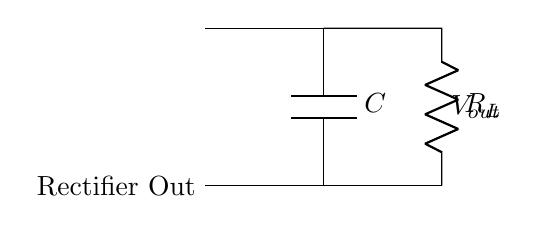
\begin{tikzpicture}[]
        \draw (0,0) node[left] {Rectifier Out} -- (3,0);
        \draw (0,2) -- (1.5,2) to[capacitor, l=$C$] (1.5,0);
        \draw (1.5,2) -- (3,2) to[resistor, l=$R_L$] (3,0);
        \node[right] at (3,1) {$V_{out}$};
    \end{tikzpicture}
    \end{answerdiagram}

    \textbf{Operation:}
    \begin{itemize}
        \item During voltage peak, capacitor charges to $V_{peak}$.
        \item During voltage drop, capacitor discharges through load, maintaining voltage.
        \item Result: Reduced ripple, smoother DC.
    \end{itemize}

    \begin{answerdiagram}{Filter Waveform}
    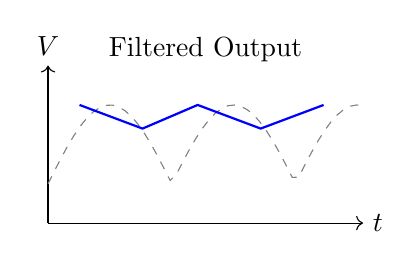
\begin{tikzpicture}
        \draw[->] (0,0) -- (4,0) node[right] {$t$};
        \draw[->] (0,0) -- (0,2) node[above] {$V$};
        \draw[gray, dashed] plot[domain=0:4, samples=50] (\x, {abs(sin(2*\x r)) + 0.5});
        \draw[thick, blue] (0.4,1.5) -- (1.2,1.2) -- (1.9,1.5) -- (2.7,1.2) -- (3.5,1.5);
        \node at (2, 2.2) {Filtered Output};
    \end{tikzpicture}
    \end{answerdiagram}

    \begin{mnemonicbox}
    \mnemonic{Capacitors Hold Voltage During Drops}
    \end{mnemonicbox}
}

\questionmarks{Question 5(a)}{3}{}
\mysolutionbox{Question 5(a)}{Define e-waste. List common e-waste items.}{
    \keyword{E-waste} (Electronic Waste) refers to discarded electrical or electronic devices that are near the end of their useful life.

    \captionof{table}{Common E-waste}
    \begin{tabulary}{\linewidth}{|L|L|}
    \hline
    \textbf{Category} & \textbf{Examples} \\
    \hline
    Computing & Laptops, PCs, Tablets \\
    \hline
    Communication & Mobile phones, Landlines \\
    \hline
    Home Appliances & TVs, Fridges, Washing Machines \\
    \hline
    Components & Batteries, PCBs, Cables \\
    \hline
    \end{tabulary}

    \begin{mnemonicbox}
    \mnemonic{Computers, Communication, Components (CCC)}
    \end{mnemonicbox}
}

\mysolutionbox{Question 5(b)}{State and explain various strategies of e-waste management.}{
    \captionof{table}{Management Strategies}
    \begin{tabulary}{\linewidth}{|L|L|}
    \hline
    \textbf{Strategy} & \textbf{Description} \\
    \hline
    Reduce & Buy less, maintain devices longer \\
    \hline
    Reuse & Repair, donate, or sell old devices \\
    \hline
    Recycle & Extract valuable metals (Au, Ag, Cu) \\
    \hline
    Disposal & Safe disposal of hazardous materials \\
    \hline
    \end{tabulary}

    \begin{mnemonicbox}
    \mnemonic{3 R's: Reduce, Reuse, Recycle}
    \end{mnemonicbox}
}

\questionmarks{Question 5(c)}{4}{}
\mysolutionbox{Question 5(c)}{Explain transistor as switch.}{
    A transistor acts as a switch by operating in \textbf{Cutoff} (OFF) and \textbf{Saturation} (ON) regions.

    \begin{answerdiagram}{Transistor Switch Circuit}
    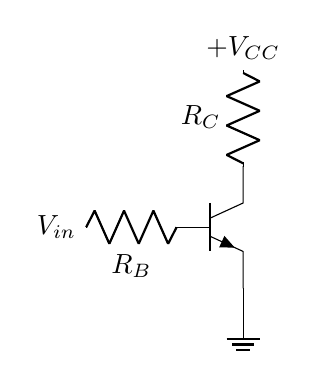
\begin{tikzpicture}[]
        \draw (0,0) node[npn] (t) {};
        \draw (t.E) -- (0,-1) node[ground] {};
        \draw (t.C) to[resistor, l=$R_C$] (0,2) node[above] {$+V_{CC}$};
        \draw (t.B) to[resistor, l=$R_B$] (-2,0) node[left] {$V_{in}$};
    \end{tikzpicture}
    \end{answerdiagram}

    \textbf{States:}
    \begin{itemize}
        \item \textbf{OFF (Open Switch)}: $V_{in} = 0V$. Base current $I_B = 0$, so Collector current $I_C = 0$. $V_{CE} = V_{CC}$.
        \item \textbf{ON (Closed Switch)}: $V_{in} = High$. $I_B$ flows, transistor saturates. $V_{CE} \approx 0V$.
    \end{itemize}

    \begin{mnemonicbox}
    \mnemonic{No Base No Current}
    \end{mnemonicbox}
}

\questionmarks{Question 5(d)}{4}{}
\mysolutionbox{Question 5(d)}{Derive relation between $\alpha$ and $\beta$ for CE configuration of transistor.}{
    \textbf{Definitions:}
    \begin{itemize}
        \item $\alpha = \frac{I_C}{I_E}$ (Common Base Gain)
        \item $\beta = \frac{I_C}{I_B}$ (Common Emitter Gain)
    \end{itemize}

    \textbf{Derivation:}
    We know that emitter current is the sum of base and collector currents:
    \begin{equation}
        I_E = I_C + I_B
    \end{equation}
    
    Divide equation (1) by $I_C$:
    $$ \frac{I_E}{I_C} = \frac{I_C}{I_C} + \frac{I_B}{I_C} $$
    $$ \frac{1}{\alpha} = 1 + \frac{1}{\beta} $$
    $$ \frac{1}{\alpha} = \frac{\beta + 1}{\beta} $$
    
    Inverting both sides:
    $$ \alpha = \frac{\beta}{1 + \beta} $$

    Rearranging for $\beta$:
    $$ \beta = \frac{\alpha}{1 - \alpha} $$

    \begin{mnemonicbox}
    \mnemonic{Beta equals Alpha over One minus Alpha}
    \end{mnemonicbox}
}

\end{document}

